\section{Kriterienbetrachtung}

Die zuvor definierten Vergleichskriterien finden nun Anwendung auf die entwickelten Apps. Die einzelnen Wertungen werden begründet, um zum Ende hin für die jeweilige App eine Kennzahl zu ermitteln, welche dann der Reflexion und der potenziellen Beantwortung der Forschungsfrage zugrunde liegen wird.

Es ist wichtig zu beachten, dass die exemplarische Entwicklung der nativen App innerhalb der iOS-Ökosystems nicht alleingestellt für die Gegenüberstellung zur \ac{pwa} verwendet werden kann. Bestimmte Aspekte können auf native Android-Entwicklung übertragen werden, andere werden wiederum außerhalb der Beispielanwendung begründet.

\subsection{Plattformabhängigkeit} \label{sec:6-plattform}
\textbf{Wertung \ac{pwa}}: $+$ \\
\textbf{Wertung native App}: $-$  \\

Um das Kriterium der Plattformabhängigkeit bewerten zu können müssen die tatsächlich unterstützten Plattformen für die \ac{pwa} zuerst geprüft werden.

\subsubsection{Browserunterstützung der \acs{pwa}}
Für Webanwendungen ist es üblich, diese mit verschiedenen Browsern zu testen. Um das Kriterium der Plattformabhängigkeit detailliert evaluieren zu können, erscheint es ebenfalls sinnvoll, die Installation der PWA sowohl auf dem Desktop, als auch auf Android und iOS Smartphones zu testen.

Zum Testen der Datenpersistenz werden Todo-Einträge angelegt und anschließend der Browser neugestartet.
Alle Browser werden mit Standardeinstellungen ausgeführt. Es werden keine Browsercaches, Cookies oder ähnliches manuell gelöscht.

\textbf{Browserunterstützung Desktop} 

\begin{table}[h!]
	\centering
	\begin{tabularx}{\textwidth}{|l||C|C|C|c|}
		\hline
		Browser              & Anwendung lauffähig & Persistente Daten & PWA installierbar & Benachrichtigungen \\
		\hline
		Chrome 78 (64-bit)   & Ja                  & Ja                & Ja                & Ja                 \\
		Firefox 70 (64-bit)  & Ja                  & Ja                & Nein              & Ja                 \\
		Edge 41    & Ja                  & Ja                & Nein              & Nein               \\
		Internet Explorer 11 & Ja                  & Ja                & Nein              & Nein               \\
		Safari 13            & Ja                  & Ja                & Nein              & Nein               \\
		\hline
	\end{tabularx}
	\caption{Browserunterstützung Desktop} \label{tab:browser_desktop}
\end{table}

Microsoft Edge und Internet Explorer zeigen den Button zum Priorisieren nicht an. Dieser enthält ein Unicodezeichen eines Sterns.

Microsoft Edge möchte die Zustimmung des Nutzers, um Benachrichtigungen anzuzeigen, zeigt jedoch anschließend keine Benachrichtigungen an. Internet Explorer wirft den JavaScript Fehler \texttt{'Notification' is undefined}, Notifications sind nicht implementiert.

\textbf{Browserunterstützung Smartphone}

\begin{table}[h!]
	\centering
	\begin{tabularx}{\textwidth}{|l||C|C|C|c|}
		\hline
		Browser           & Anwendung lauffähig & Persistenz & PWA installierbar & Benachrichtigungen \\
		\hline
		\multicolumn{5}{|c|}{Android}                                                                 \\
		\hline
		Chrome 78         & Ja                  & Ja         & Ja                & Ja                 \\
		Firefox 68        & Ja                  & Ja         & Ja                & Ja                 \\
		Edge 41 & Ja                  & Ja         & Nein              & Ja                 \\
		Opera 54          & Ja                  & Ja         & Nein              & Ja                 \\
		\hline
		\multicolumn{5}{|c|}{iOS}                                                                     \\
		\hline
		Chrome            & Ja                  & Ja         & Nein              & Nein               \\
		Safari 13         & Ja                  & Ja         & Nein              & Nein               \\
		\hline
	\end{tabularx}
	\caption{Browserunterstützung Smartphones} \label{tab:browser_smartphones}
	
\end{table}


Verweigert der Nutzer die Benachrichtigungen einer Webseite, ist es meist umständlich die Berechtigung für Benachrichtigungen einer Website zurückzusetzen. Beim Browser Opera muss der Nutzer dann beispielsweise durch fünf Menüs nacheinander navigieren, um die deaktivierten Benachrichtigungen wieder zu aktivieren.

\subsubsection{Bewertung \ac{pwa}}
Die Praxis zeigt, dass die Webanwendung zwar plattformübergreifend auf iOS, Android und Desktop funktioniert, aber nur Android Nutzer von der Installierbarkeit der \ac{pwa} profitieren.
Hier soll ein Vergleich zur nativen iOS App geschlossen werden. Beide unterstützen die Installation auf einer mobilen Plattform, die \ac{pwa} bietet jedoch auch die Nutzung im Web für iOS Geräte und eine installierbare Anwendung für Desktopgeräte und ist damit in diesem Kriterium der nativen App überlegen. Das Kriterium wird mit eher gut, aber nicht mit gut bewertet, da die \ac{pwa} nicht auf Apple Mobilgeräten installiert werden kann.

\subsubsection{Bewertung native App}
Die iOS-Anwendung findet in einem geringen Rahmen Anwendung. Somit kann diese nur auf einem relativ geringen Anteil der führenden Mobilgeräte verwendet werden. Anders als bei der \ac{pwa} kann auch keine limitierte Nutzung gewährleistet werden. An dieser Stelle greift auch kein Argument, welches sich auf die Exemplarität der nativen Entwicklung bezieht. Für die Nutzung verschiedener Plattformen in ihrer nativen Form müsste eine App mehrmals entwickelt werden. Diese Erkenntnis würde auch bei der Umsetzung der Beispielanwendung unter Android greifen, mit der Ausnahme, dass Android-Apps untereinenander eine deutlich höhere Geräteunabhängigkeit aufweisen, da Android von einer Vielzahl Smartphoneherstellern unterstützt wird, während iOS nur unter der eigenen Marke zur Anwendung kommt. Es existieren zwar Frameworks, welche die plattformübergreifende Entwicklung von Apps und deren native Bereitstellung in den entsprechenden Bezugspunkten erlauben (bspw. das JavaScript-Framework ReactJS), jedoch entfällt dieses aus dem Betrachtungsrahmen dieser Arbeit. Außerdem müssten auch dort Änderungen vollzogen werden, die sich in den Unterschieden der Benutzeroberflächen der einzelnen Betriebssysteme begründen. Das Kriterium wird hier mit eher schlecht bewertet. Die Bewertung schlecht kommt nicht zum Einsatz, da die Apps in ihrem Ökosystem trotzdem ausnahmslos geräteübergreifend funktionieren.

\subsection{Installation} \label{sec:6-installation}
\textbf{Wertung \ac{pwa}}: \Circle \\
\textbf{Wertung native App}:  \\

\subsection{\ac{pwa}}
Die \ac{pwa} wird über den Browser installiert. Daher ist die Installation stark abhängig vom verwendeten Browsertyp. Teilweise ist die Installation der Anwendung bedingt durch den Browser überhaupt nicht möglich. Bezogen auf den Desktopbrowser Chrome dürfte es der Praxis häufig vorkommen, dass Nutzer die Bedienelemente zur Installation im Browser nicht als solche wahrnehmen (Siehe Abbildung \ref{fig:dialog_install_pwa_desktop}).Dies wird als negativ gewertet.

Die Installation ist für den Nutzer transparent. Er sieht nicht, dass beziehungsweise wie viele Daten bereits heruntergeladen wurden. Der ein oder andere Nutzer wird sich möglicherweise nicht bewusst sein, dass \texttt{zum Startbildschirm hinzufügen} eigentlich eine Installation ausführt.

Die Installation dauert je nach Komplexität der Webanwendung keine ganze bis wenige Sekunden.

Die Deinstallation auf Android Geräten erfolgt wie bei nativen Apps. Bei der Desktop \ac{pwa} ist diese unter Windows sogar deutlich einfacher, als bei Desktopanwendungen.

Insgesamt ist die Installation einer \ac{pwa} sehr einfach und mit nur einem Befehl des Nutzers ausführbar. Das gilt aber nur dann, wenn der Nutzer das Konzept der \ac{pwa} begriffen hat, was nach heutigem Stand wohl nicht der Fall sein dürfte. Die Installation selbst kommt ohne Lizenzvereinbarungen oder Installationspfade daher und ist außerdem bemerkenswert schnell.

Da einige störende Punkte für den Nutzer nicht optimal sind, die Installation insgesamt aber ein einfacher Prozess ist, erhält dieses Kriterium eine neutrale Wertung.


\subsection{Speicherzugriff} \label{sec:6-speicherzugriff}
\textbf{Wertung \ac{pwa}}: $+$\\
\textbf{Wertung native App}: $++$ \\

\subsubsection{Bewertung \ac{pwa}}
Die \ac{pwa} hat keinen Zugriff auf das Dateisystem. Daten werden über den Browser im Speicher abgelegt, beispielsweise im Key-Value-Store \texttt{local storage}. Konfigurationen und Daten können auf diese Weise einfach gespeichert werden.

Das Speichern von binären Daten, wie Bildern, gestaltet sich in der Praxis als schwierig. Es existieren uneinheitliche browserspezifische Lösungen. Höchstwahrscheinlich kommt der Entwickler aber nicht um das Speichern binärer Daten als kodierter Text, wie beispielsweise Base64.

Das Kriterium wird als eher gut bewertet, weil mit dem Browserspeicher ein Großteil der Anwendungsfälle für Datenspeicherung abgedeckt ist und diese sehr einfach von Entwickler genutzt werden können.

\subsubsection{Bewertung native App}
Die Beispielanwendung nutzt die Bibliothek \texttt{CoreData}, welche es erlaubt, zu speichernde Dateistrukturen in Form von Datenbank-Design anzulegen und in den Benutzungsrahmen der App hinzuzufügen. Innerhalb der Android-Entwicklung existieren verschiedene Formen app-bezogenen Speichers, welche für unterschiedliche Zwecke verwendet werden können. In beiden Fällen bedarf es \textit{Endpoints}, welche das Verhalten des Speicherzyklus definieren.

Durch eine Speicherarchitektur, welche an relationale Datenbanken erinnert, können auch komplexe Speicherstrukturen entstehen, bspw. über die Definition verschiedener Speicherareale, welche in der Beispielanwendung keinen Nutzen fanden. Anders als bei \acp{pwa} existieren keine Einschränkungen von Dateiformaten.

Das Kriterium kann somit uneingeschränkt als gut bewertet werden, da zumindest in der Beispielanwendung keinerlei Grenzen des Speicherzugriffes aufgedeckt werden konnten.

\subsection{Speicherbedarf} \label{sec:6-speicherbedarf}
\textbf{Wertung \ac{pwa}}: $++$ \\
\textbf{Wertung native App}: $+$ \\

\subsection{\ac{pwa}}
Die implementierte Anwendung hat einen bemerkenswert kleinen Speicherbedarf von  nur 430 Kilobyte. Verglichen mit einer üblichen nativen Implementierung, die sich im Bereich mehrerer Megabyte bewegt, wird dieses Kriterium mit sehr gut bewertet.

\subsection{Bewerung native App}
Nach direkter Installation der Anwendung geben die Speicherinformationen der Systemeinstellungen des Testgerätes einen Bedarf von insgesamt 475 Kilobyte an. Pro To-Do-Eintrag wächst dieser um ca. 50 Kilobyte. Es lässt sich keine genaue Schätzung für eine äquivalente Android-App ableiten, weswegen dieser Gesichtspunkt wegfällt.

Da sich die native App auf Augenhöhe mit der \ac{pwa} befindet, jedoch einen hohen Bedarfszuwachs erfordert, wenn auf den Speicher der App geschrieben wird, wird dieses Kriterium mit eher gut bewertet.

\subsection{Aktualisierbarkeit} \label{sec:6-aktualisierbarkeit}
\textbf{Wertung \ac{pwa}}: $++$ \\
\textbf{Wertung native App}: $+$ \\

\subsection{\ac{pwa}}
Der Browser beziehungsweise der laufende Service-Worker verwaltet das Caching und die Aktualisierung der Anwendung. Für den Nutzer sind Aktualisierungen transparent. Er muss ihnen nicht zustimmen und kann sie nicht vermeiden. 

Entwickler müssen nur die neue Version der Anwendung deployen, damit die Installationen auf den Nutzergeräten aktualisiert werden.

Weil vom Nutzer keine Aktion erforderlich ist und die Aktualisierung für Entwickler sehr einfach ist, erhält dieses Kriterium eine sehr gute Wertung.

\subsection{Bewertung native App}
Wie auch bei der Installation administriert der zentrale Bezugspunkt (Apple App Store resp. Google Play Store) auch die Aktualisierung der auf dem Gerät installieren Apps. Je nach Nutzereinstellungen werden diese automatisch bezogen oder der Nutzer wird benachrichtigt, dass Updates verfügbar sind.

Wie bereits erwähnt werden alle Aktualisierungen, welche vom Entwickler vertrieben werden, vor Veröffentlichung erneut geprüft. Dies stellt einen Vor- wie einen Nachteil dar. Grundsätzlich kann aufgrund des Qualitätsmanagements der Bezugspunkte von einer sicheren Distribution ausgegangen werden. Andererseits können relevante Hotfixes dadurch auch verzögert werden. Sollte der Nutzer die automatischen Updates deaktiviert haben, so kann es sein, dass dieser sicherheitsrelevante Aktualisierungen nicht mitbekommt oder bewusst ignoriert, was nicht im Sinne der Entwickler ist.

Verglichen mit \acp{pwa} kann der Nutzer alle Updates genau nachverfolgen, da parallel zu diesen auch Informationen über die neuen Inhalte, Bug-Fixes, etc. veröffentlicht werden können. Sollte eine Sicherheitslücke einer neuen Version bekannt werden, so kann der Nutzer diese ignorieren, bis eine weitere Version veröffentlicht wird, welche diese behebt.

Alles in allem gewinnen gewisse Pro- bzw. Contra-Argumente an Bedeutung, je nachdem, welche Position gerade betrachtet wird. Zusammengefasst kann die Aktualisierbarkeit aber mit eher gut bewertet werden, da der Prozess an sich funktioniert und für den Nutzer in jeder Hinsicht transparent ist, jedoch unter gewissen Umständen ignoriert werden kann.

\subsection{Design} \label{sec:6-konsistenz-des-designs}
\textbf{Wertung \ac{pwa}}: $-$\\
\textbf{Wertung native App}: $+$ \\

\subsection{\ac{pwa}}
Das Aussehen der Anwendung wird maßgeblich durch die Browserengine bestimmt, welche HTML und CSS rendert. Es ist seither ein bekanntes Problem, dass CSS von verschiedenen Browsern unterschiedlich interpretiert wird und es für viele Features keine einheitliche Unterstützung gibt.

Nicht zuletzt liegt es aber am Entwickler, der große Teile des Implementierungsaufwands für das Design an Frameworks und Bibliotheken abgeben kann, um ein konsistentes Design zu erzeugen. 

Schließlich gibt es Webanwendungen und Designanforderungen bereits seit einigen Jahren, sodass für die meisten trivialen Probleme bereits Lösungen bestehen.

Dieses Kriterium wird als negativ bewertet, da das Stylen mit CSS zwar mit großen Freiheiten aber auch deutlichen Konsistenzproblemen einhergeht.

\subsection{Bewertung native App}
Die Abhängigkeit gegenüber der geschlossenen Plattform iOS erlaubt es der Entwicklungsoberfläche und auch Apple selbst, bestimmte Richtlinien für ein konsistentes und konformes Design einzuführen und zu erzwingen. Durch die Suggestion bestimmter, bereits vordefinierter Komponenten während der Entwicklung wird dem Entwickler ein großer Teil der Gestaltungsarbeit abgenommen. Animationen, der vordefinierte Aufbau komplexer Komponenten, etc., benötigen nur wenige Quellcodezeilen für die Umsetzung und können teilweise auch komplett visuell über Interface Builder angelegt werden. Die teils erzwungene Konsistenz lässt sich zwar positiv für das Gesamtbild werten, stellt jedoch Hürden bezüglich der Kreativität des Entwicklers dar; für den Fall, dass eigene Animationen oder Komponentenstrukturen gewünscht sind, so sind diese sehr aufwändig zu definieren und umzusetzen. Es lässt sich deuten, dass dies unter der Android-Entwicklung nicht anders zur Geltung kommt.

Die Plattformabhängigkeit erlaubt aufgrund weniger, unterschiedlicher Bildschirmgrößen eine übersichtliche Möglichkeit, die Skalierung der Komponenten auf verschiedenen Geräten dynamisch zu gestalten. Durch die Vielzahl an unterstützten Android-Geräten lässt sich interpretieren, dass sich die Einhaltung einer solchen Konsistenz dort schwieriger gestaltet.

Die Designumsetzbarkeit stellt sich v.a. im Vergleich zu \acp{pwa} deutlich aufwandsfreier dar, jedoch bringen vor allem Kreativitätshürden durch Design-Suggestionen und die evtl. komplexe Dynamisierung der Komponentenposition unter Android nicht vernachlässigbare Schwächen mit, weswegen das Kriterium insgesamt mit eher gut bewertet wird.

\subsection{Bibliotheken} \label{sec:6-bibliotheken}
\textbf{Wertung \ac{pwa}}: $++$\\
\textbf{Wertung native App}: $+$ \\

\subsubsection{\ac{pwa}}
Frameworks und Bibliotheken für JavaScript gibt es sprichwörtlich zu Tausenden. In der Praxis ist es ausgesprochen selten zu einem Problem keine existierende (Teil-)Lösung in Form eines npm Pakets zu finden.

Die Nutzung und Installation dieser Pakete ist mit dem npm Paketmanager einfach, automatisierbar und dürfte einen großen Teil zur Wahl der Programmiersprache JavaScript beitragen.

Dieses Kriterium ist eindeutig mit sehr gut zu werten.

\subsubsection{Bewertung native App}
Apple bietet für Swift eine Vielzahl von Bibliotheken an, eine Ergänzung bieten Drittanbieterbibliotheken, welche ebenfalls in die Entwicklungsumgebung eingebunden werden können. Gerade die direkte Unterstützung der eigenen Bibliotheken ermöglicht eine nahtlose Inklusion in den gesamten Entwicklungszyklus. Jedoch ist JavaScript wesentlich verbreiteter als Swift, weswegen das Volumen vorhandener Bibliotheken, welche die Entwicklung vereinfachen, deutlich größer ist. Die Android-Entwicklung ist jedoch ebenfalls sehr verbreitet, weswegen gerade dafür ebenfalls eine Vielzahl von Bibliotheken zur Verfügung steht. Da die bloße Anzahl der insgesamt vorhandenen Bibliotheken der einzige Punkt ist, in welchem die native Entwicklung der Webentwicklung (und somit der \ac{pwa}-Entwicklung) nachsteht, kann das Kriterium mit eher gut bewertet werden.

\subsection{Umsetzbarkeit} \label{sec:6-umsetzung}
\textbf{Wertung \ac{pwa}}: $++$\\
\textbf{Wertung native App}: $++$ \\

\subsection{\ac{pwa}}
Die Kombination aus dem Framework Angular, einer \ac{pwa} und der Hostinglösung Firebase funktioniert in der Praxis bemerkenswert reibungslos.

Angular reduziert den Implementierungsaufwand gegenüber vanilla JavaScript durch saubere Strukturierung der Anwendung in Komponenten und Services.

In der Praxis war es nicht möglich, Benachrichtigungen ohne Netzwerkverbindung zu senden. Das ist ein großes Manko im Vergleich zur nativen App.

Das Testen der \ac{pwa} war lokal nicht möglich beziehungsweise mit nicht vertretbarem Aufwand realisierbar.

Dieses Kriterium ist mit sehr gut zu werten.

\subsection{Bewertung native App}
Im Punkto Umsetzbarkeit konnten alle Anforderungen der in Kapitel 3 definierten Architektur realisiert werden. Durch die durchgehende Nutzung der durch Apple empfohlenen Architekturstruktur MVC war dies auch ohne größeren Aufwand oder die zwingende Nutzung von Umwegen möglich.

Im abgegrenzten Rahmen der Umsetzbarkeit wurden alle Anforderungen erfüllt, weswegen das Kriterium als gut bewertet werden kann.

\subsection{Testbarkeit} \label{sec:6-testbarkeit}
\textbf{Wertung \ac{pwa}}: sehr gut\\
\textbf{Wertung native App}:  \\

\subsection{\ac{pwa}}
Ein Vorteil, welchen das JavaScript Ökosystem mit seinen Frameworks und Bibliotheken mit sich bringt, ist die Vielzahl existierender Testlösungen für beispielsweise Unittesting.

Ein gravierender Vorteil gegenüber nativer Apps ist, dass Entwickler die Anwendung im Desktopbrowser testen können und keinen Android/iOS Emulator benötigen. Dahingehend ist das Testen der Anwendung deutlich einfacher, schneller und ressourcenschonender.

Die Testbarkeit wird deshalb mit sehr gut bewertet.

\subsection{Vorausgesetzte Entwicklungserfahrung} \label{sec:6-vorausgesetzte-entwicklungserfahrung}
\textbf{Wertung \ac{pwa}}: $-$\\
\textbf{Wertung native App}: $+$ \\

\subsubsection{Bewertung \ac{pwa}}
Die \ac{pwa} setzt sich aus drei programmiersprachlichen Komponenten zusammen: JavaScript, HTML und CSS. Damit erfordert die Entwicklung sowohl Kenntnisse in prozeduraler Programmierung, als auch in der Implementierung passender HTML und CSS Strukturen, welche letztendlich nur durch JavaScript modifiziert werden.

Außerdem ist zu erwähnen, dass komplexe JavaScript Anwendungen ohne Frameworks und Bibliotheken in der Praxis selten zu finden sind. Die Nutzung von JavaScript ohne beispielsweise Angular, React oder Vue.js ist mit nicht vertretbarem Aufwand verbunden. Da die Nutzung eines Frameworks quasi notwendig ist, aber es zwischen jenen deutliche Unterschiede gibt, zählt dies ganz klar zu den Wissensvoraussetzungen.

Dazu kommen auch zwingend Kenntnisse der Linux-Kommandozeile für node.js, npm und wahrscheinlich eines \ac{cli}-Tools für das Deployment.

Die Wissenshürde ist deutlich erkennbar und für erfahrene Programmierer ohne Webkenntnisse dennoch vorhanden. Dieses Kriterium wird als negativ eingestuft.  

\subsubsection{Bewertung native App}
Die Entwicklung einer iOS-App geschieht grundsätzlich innerhalb der Programmiersprache Swift. Diese greift jedoch auf Paradigmen des Vorgängers Objective-C zurück. Es werden zwar umfassende Kenntnisse \textit{nur} einer Programmiersprache benötigt, jedoch ist diese in ihrer Tragweite sehr umfangreich und folgt nicht immer den üblichen Entwicklungsmustern. Die Beispielanwendung lies sich ohne jegliche Drittanbieter-Bibliotheken umsetzen, weswegen die benötigten Dokumentationen der genutzten Funktionen überwiegend vom Betreiber Apple stammen, was zur Korrektheit und Aktualität dieser beiträgt. Positiv anzumerken ist ebenfalls die Tatsache, dass v.a. \ac{ui}-Konfigurationsschritte über Interface Builder vereinfacht bzw. ersetzt werden können. Dies ist ebenfalls auf die Android-Entwicklung zu beziehen.

Da die Entwicklung in nativen Umgebungen durch verschiedene Lösungen vereinfacht wird und verglichen mit \acp{pwa} sich in einem Umfeld aufhält, werden insgesamt weniger Voraussetzungen an den Entwickler gestellt. Auf der anderen Seite handelt es sich um sehr umfangreiche Programmierumgebungen, weswegen eine gewisse Erfahrung von Vorteil sein könnte. Insgesamt ist dieses Kriterium also mit eher gut zu bewerten.

%\section{Nutzerfreundlichkeit} \label{sec:6-verstaendlichkeit}
%\textbf{Wertung \ac{pwa}}: gut\\
\textbf{Wertung native App}:  \\



\subsection{\ac{pwa}}


\section{Gesamtbetrachtung}
Für die Gesamtbetrachtung werden die Ergebnisse zur besseren Übersicht erneut in der Evaluationsmatrix (Tabelle \ref{tab:evaluationsmatrix_ausgefüllt}) dargestellt. Die Bewertung befindet sich im Bereich 2,0 ($++$ oder gut) und $-$2,0 ($--$ oder schlecht). 0,0 Verrechnungspunkte bilden die neutrale Mitte (\Circle).

 In der gewichteten Summe erhält die \ac{pwa} 0,55 Verrechnungspunkte. Das entspricht einer Wertung zwischen neutral (\Circle) und eher gut ($+$). Die native App erhält in der gewichteten Summe 1,1 Verrechnungspunkte, was einer eher guten Wertung entspricht ($+$).

\begin{table}[h!]
	\centering
	\begin{tabular}{|l|c|c|c|}
		\hline
		Kriterium              & Gesamtanteil & \cellcolor{green!25}\ac{pwa} & \cellcolor{blue!25} native App\\
		
		\hline
		\multicolumn{4}{c}{Anwendung}         \\
		\hline
		Plattformabhängigkeit   & 10\%         & \cellcolor{green!25}$+$ &\cellcolor{blue!25}$-$\\
		Installation           & 5\%          & \cellcolor{green!25}\Circle & \cellcolor{blue!25}$++$ \\
		Speicherzugriff        & 5\%          & \cellcolor{green!25}$+$&\cellcolor{blue!25}$++$ \\
		Speicherbedarf         & 5\%          &\cellcolor{green!25}$++$&\cellcolor{blue!25}$+$\\
		Aktualisierbarkeit     & 5\%          &\cellcolor{green!25}$++$&\cellcolor{blue!25}$+$ \\
		Konsistenz des Designs & 5\%         & \cellcolor{green!25}$-$&\cellcolor{blue!25}$+$\\
		
		\hline
		\multicolumn{4}{c}{Entwicklung}      \\
		\hline
		Bibliotheken           & 10\%         &\cellcolor{green!25}$++$&\cellcolor{blue!25}$+$ \\
		Umsetzung              & 20\%         &\cellcolor{green!25}$+$&\cellcolor{blue!25}$++$ \\
		Testbarkeit            & 10\%         &\cellcolor{green!25}$++$&\cellcolor{blue!25}\Circle\\
		Vorausgesetzte Entwicklungserfahrung    & 10\%  &\cellcolor{green!25}$-$&\cellcolor{blue!25}$+$ \\
		\hline
		\hline
		Gesamt                  & 100\%        & \cellcolor{green!25}0,55 (\Circle/$+$) &\cellcolor{blue!25}1,1 ($+$)\\
		\hline
	\end{tabular}
	\caption{Ergebnisse in der Evaluationsmatrix} \label{tab:evaluationsmatrix_ausgefüllt}
\end{table}

Die einzelnen Kriterien werden im Netzdiagramm (Abbildung \ref{fig:netzdiagramm}) visualisiert. Bei der Wertung ist zu beachten, dass die einzelnen Kriterien zwar gewichtet einfließen, jedoch gibt es unterschiedliche Interpretationsweisen für die einzelnen Kriterien. Diese Arbeit befindet sich dabei meist auf dem Standpunkt des Entwicklers und gewichtet die Anforderungen der Nutzer entsprechend geringer. Andere Forschungsansätze würden bei anderen Forschungsschwerpunkten zu abweichenden Interpretationen und Ergebnissen führen.
%	Plattformabhängikeit   & 0   & 1 & 2       & 3 & 4  & 10\%         \\
%Installation           & 0   & 1 & 2       & 3 & 4  & 5\%          \\
%Speicherzugriff        & 0   & 1 & 2       & 3 & 4  & 5\%          \\
%Speicherbedarf         & 0   & 1 & 2       & 3 & 4  & 5\%          \\
%Aktualisierbarkeit     & 0   & 1 & 2       & 3 & 4  & 5\%          \\
%Konsistenz des Designs & 0   & 1 & 2       & 3 & 4  & 5\%         \\
%Bibliotheken           & 0   & 1 & 2       & 3 & 4  & 10\%         \\
%Umsetzung              & 0   & 1 & 2       & 3 & 4  & 20\%         \\
%Testbarkeit            & 0   & 1 & 2       & 3 & 4  & 10\%         \\
%Vorausgesetzte Entwicklungserfahrung    & 0   & 1 & 2       & 3 & 4  & 10\%         \\
%Verständlichkeit       & 0   & 1 & 2       & 3 & 4  & 10\%         \\
%
\begin{figure}[h]

	\begin{tikzpicture}
	
		% Diagram setup
		\tkzKiviatDiagram[scale=1.0,label distance=.5cm,
		radial  = 4,
		gap     = 1,  
		lattice = 4]{
			Plattformabhängigkeit,
			Installation,
			Speicherzugriff,
			Speicherbedarf,
			Aktualisierbarkeit,
			Designs,
			Bibliotheken,
			Umsetzung,
			Testbarkeit,
			Vorausgesetzte Entwicklungserfahrung,
			Nutzerfreundlichkeit
		}
		
		% native App
		\tkzKiviatLine[thick,color=blue,mark=ball,
		fill=blue!20,opacity=.5](2,4,4,2,3,3,1,2,3,3,4)
		
		% PWA
		\tkzKiviatLine[thick,color=green,mark=ball,
		fill=green!20,opacity=.5](3,2,3,4,4,1,4,4,4,1,2)
		
		\tkzKiviatGrad[prefix=,unity=1,suffix=](0)  
	

	
	\end{tikzpicture}
	
	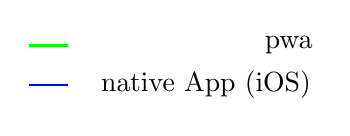
\begin{tikzpicture}
	%\draw[draw=black!20] (-0.1,-0.2) rectangle ++(15,0.5);
	
	\draw [thick, green] (0,0.5) -- (0.5,0.5); 
	\node at (3.3,0.5) {\acf{pwa}};
	
	\draw [thick, blue] (0,0) -- (0.5,0); 
	\node at (2.25,0) {native App (iOS)};
	

		\end{tikzpicture}
	
	\caption{Spinnennetzdiagram: Kriterienvergleich \acs{pwa} und native App}
\end{figure}

\section{Fazit}

Ob sich die \ac{pwa} etablieren kann steht und fällt mit der zukünftigen Unterstützung durch Browserhersteller insbesondere Apples Safari aufgrund seiner hohen Marktverbreitung. Es ist davon auszugehen, dass die Mehrheit der Nutzer ihren Browser nicht nach Kriterien der JavaScript-Unterstützung wählt und sie für die Nutzung von \ac{pwa}s keinen neuen Browser herunterladen.

Es ist nach den Erkenntnissen dieser Arbeit jedoch fraglich, ob sich Apple grundsätzlich weiter mit \ac{pwa}s beschäftigt. Das Konzept bietet für Entwickler großes Potenzial, da verglichen mit nativer Implementierung häufig eine doppelte Programmierung für Web und Apps entfällt. Aber gerade deshalb steht die \ac{pwa} in Konkurrenz zu Apples AppStore. Mit der Entscheidung \ac{pwa}s zu unterstützen, gibt ein Hersteller die Kontrolle über die auf seinen Geräten installierten Apps ab. 
Möglicherweise würde man einen lukrativen Markt, den Verkauf von Software/Apps, in die Hände einzelner Unternehmen geben.

Für Entwickler jedenfalls wäre dies erfreulich, da im Hinblick auf die schnelle Ausbreitung von JavaScript im Webbereich quasi für jedes Problem bereits eine Lösung existiert. Nicht zuletzt kommuniziert fast jede native App sowieso mit dem Internet, um dynamisch Daten zu laden und zu speichern. Ein Webentwickler könnte mit einer \ac{pwa} eine App entwickeln, ohne Spezialist für eine Plattform zu sein. Unter Verwendung von Node.js könnten App, Website und Webservices alle in der gleichen Sprache, JavaScript, entwickelt werden.

Bezieht man sich bei der Reflexion ausschließlich auf Anwendungen im Web, würden die meisten Webseiten von den Caching-Möglichkeiten der \ac{pwa} profitieren, Ladezeiten verkürzen können und dem Nutzer ein flüssigeres Gesamterlebnis bieten. Es ist davon auszugehen, dass sich das positiv auf die Kundeninteraktionen mit der Website auswirkt.
